


In order to create a basis for the engine choice, a trade study was performed on the engines of similar aircraft. These aircraft, such as the Boeing 777-300, Airbus A330-300, Airbus A330-900, and Airbus A350 XWB, have a similar passenger capacity as the one required in the design competition, however all have a much higher range capability. The primary drivers for the design of the propulsion system are the power requirement for the aircraft, as well as reliability. Since the aircraft will be used as a high capacity transport for short mission durations, it is vital that the engines can withstand a constant cycle of maximum take off thrust at a higher interval than tradition engines which experience longer flight durations. 

\subsection{Engine Comparisons}

The following engines, seen below, are used in similar aircraft with great success: Pratt \& Whitney PW4000, General Electric GE90-115B, Rolls-Royce Trent XWB, and Rolls-Royce Trent 7000.

\begin{table}[!h]
    \centering
        \caption{Comparison of Engines on Similar Aircraft}
    \begin{tabular}{|c||c|c|c|c|}\toprule
         & \textbf{PW4000} & \textbf{GE90-115B} & \textbf{RR Trent XWB} & \textbf{RR Trent 7000} \\\hline \hline
         \textbf{Aircraft} & Airbus A330-300 & Boeing 777-300 & Airbus A350 XWB & Airbus A330-900\\ \hline
         \textbf{Maximum Takeoff Thrust} & 52,000 - 62,000 lbs \cite{PW} & 110,000 lbs \cite{ge90} & 84,200 lbs \cite{xwb} & 71,110 lbs \cite{butterworth}\\ \hline
         \textbf{Dry Weight} & 12,900 lbs \cite{FAApw} & 19,316 lbs \cite{ge90} & 16,043 lbs \cite{xwb2} & 10,550 \cite{butterworth} \\ \hline
         \textbf{Cost per Unit} & - & \$ 27.5 million \cite{gecost} & - & \$ 11 million \cite{butterworth} \\ \hline
         \textbf{Bypass Ratio} & 4.9 \cite{PW} : 1 \cite{PW} & 9 \cite{safran} & 9.6 : 1 \cite{xwb} & 4.89 : 1 \cite{butterworth} \\ \hline
         \textbf{Fan Diameter [in]} & 94 \cite{PW} & 135 \cite{ge} & 118 \cite{xwb} &  97 \cite{butterworth}\\ \hline
         \textbf{Thrust to Weight} & 4.80-4.03 & 5.69 & 5.24 & 6.74 \\ \bottomrule
    \end{tabular}
    \label{tab:enginecomp}
\end{table}

While the aircraft are similar in capacity, the range on these aircraft is much higher than what is required for the Sam Mark I. As such, an assumption is made that the engines chosen for these aircraft may not be as reliable as necessary for the Sam Mark I, since the engine for the Sam Mark I will experience higher intervals and much more frequent cycling of maximum thrust, leading to more fatigue to the engine. 

In order to validate our choice of a turbofan engine, which was also the type of engine of choice for the similar aircraft compared above, Figure ~\ref{PropSelection} was used along with the Mach speed the Sam Mark I will fly at cruise conditions, 0.9. This figure was used to quickly determine which propulsion systems are overpowered for the flight conditions that the aircraft will fly and rule out which propulsion systems would not be able to meet the flight conditions.

\begin{figure} [h!]
    \centering
    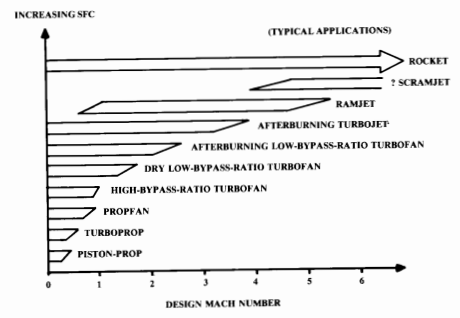
\includegraphics[width=0.8\textwidth]{Photos/PropSelection.PNG}
    \caption{Propuslion system speed limits. \cite{raymer}}
    \label{PropSelection}
\end{figure}

\newpage
With a Mach number of 0.9, both piston-prop and turboprop engines are not able to meet the speed requirement for cruise. The propfan propulsion system, while it may be able to handle a Mach number of 0.9, is not ideal as it is operating at the end of its limit. Scramjet and ramjet propulsion systems are over powered for the Sam Mark I system, leaving only three classes of turbofan engines and an afterburning turbojet engine. According to Raymer, the propulsion system should be one which the lowest on the chart for the specified Mach number, which for our case is the high-bypass-ratio turbofan \cite{raymer}. In addition, all of the engines listed in Table \ref{tab:enginecomp} are high-bypass-ratio turbofan propulsion systems as well, which gives confidence in the high-bypass-ratio turbofan engine being the propulsion system of choice for the Sam Mark I, barring any critical design concerns.


\subsection{Future Progress}

To solidify an engine choice, the sizing requirements and values that were generated by the team will be used to form a power requirement guideline for the propulsion system. This power requirement will be the primary driver for the choice of an engine as it will ensure that the engine chosen is not overpowered and that it will perform as necessary. Taking into account the need for the engine to be highly reliable as it may experience higher rates of fatigue due to the short mission, reliability will be the secondary driver for the propulsion system. The cost will be considered as well, however it will not be as prioritized as the goal is to design and choose as reliable of a system as possible.


%% Or...:
% \begin{wrapfigure}{r}{0.5\textwidth}
%     \centering
%     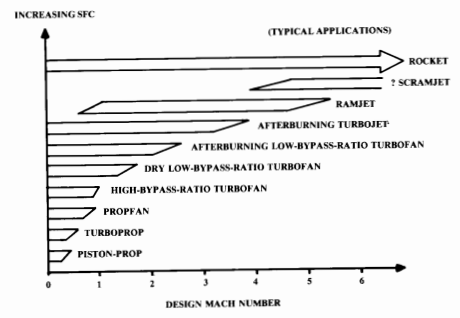
\includegraphics[width=0.5\textwidth]{Photos/PropSelection.PNG}
%     \caption{Caption}
%     \label{fig:my_label}
% \end{wrapfigure}

% \textcolor{red}{
% \begin{itemize}
%     \item Discuss overall propulsion system philosophy/design/selection.
%     \item Discuss future work.
%     \item AIAA: Propulsion system description and characterization including performance,
%     dimensions, and weights. The selection of the propulsion system(s), sizing, and
%     airframe integration must be supported by analysis, trade studies, and discussion
% \end{itemize}}